\documentclass[10pt,t]{beamer}
\usetheme{desynew}
\setbeamertemplate{second logo in title page}[desy]

\usepackage[utf8]{inputenc}
\usepackage[T1]{fontenc}
\usepackage{textcomp}
\usepackage[english]{babel}
\usepackage{microtype}
\usepackage{tikz}
\usetikzlibrary{positioning,calc}

\graphicspath{{images/}{bilder/}}

\title[Welcome at DESY]{Welcome at DESY!}
\author[Joscha Knolle]{\textbf{Joscha Knolle}}
\institute{PhD Student (particle physics)\\DESY CMS group\\[\baselineskip]Introductory lecture for Viborg Katedralskole}
\date[04 Dec 2019]{December 4th, 2019}

\def\Put(#1,#2)#3{\leavevmode\makebox(0,0){\put(#1,#2){#3}}}
\unitlength=0.01\paperwidth

\begin{document}

\maketitle


\begin{frame}
\frametitle{What is DESY?}
\vspace*{-2\baselineskip}
\begin{columns}[c]
\column{0.472\textwidth}\begin{itemize}
    \item \textbf{D}eutsches \textbf{E}lektronen-\textbf{Sy}nchrotron
    \item national research centre
    \item member of Helmholtz Association
    \item established on December 18th, 1959
    \item two locations:
    \begin{itemize}
        \item Hamburg
        \item Zeuthen (Brandenburg)
    \end{itemize}
    \item budget: 230 million euro (2016)
    \begin{itemize}
        \item 90\,\% federal government
        \item 10\,\% state governments of Hamburg \& Brandenburg
    \end{itemize}
\end{itemize}
\column{0.472\textwidth}
    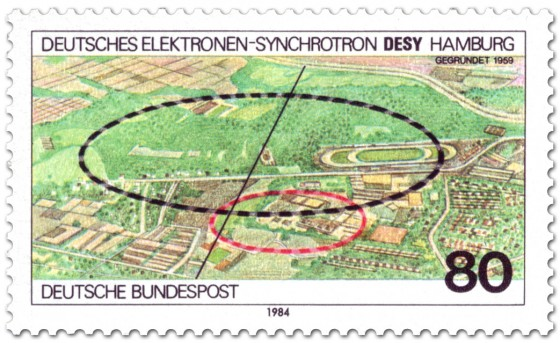
\includegraphics[width=\textwidth]{briefmarke} \\[1ex]
    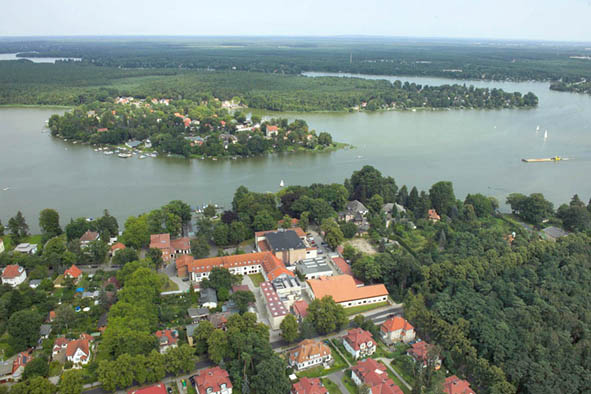
\includegraphics[width=\textwidth]{zeuthen}
\end{columns}
\end{frame}


\begin{frame}
\frametitle{Helmholtz Association}
\framesubtitle{Helmholtz Association of German Research Centres}
\vspace*{-1.5\baselineskip}
\begin{itemize}
    \item Germany's largest scientific organisation
    \begin{itemize}
        \item more than 39,000 employees in 19 research centres
        \item budget: 4.5 billion euro (2018)
    \end{itemize}
    \item long-term basic research to solve the major challenges facing society, science and the economy
    \item research fields:
\end{itemize}

\begin{tikzpicture}
    \node [inner sep=0pt] at (0,0) {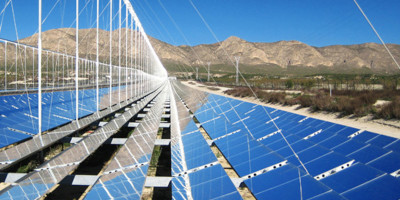
\includegraphics[width=0.3\textwidth]{fb-energie}};
    \node [inner sep=0pt] at (0.35\textwidth,0) {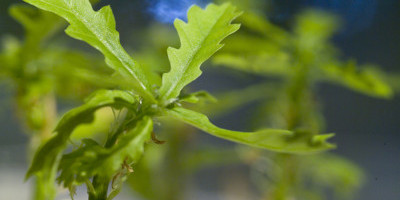
\includegraphics[width=0.3\textwidth]{fb-erdeumwelt}};
    \node [inner sep=0pt] at (0.7\textwidth,0) {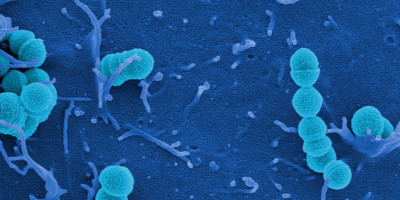
\includegraphics[width=0.3\textwidth]{fb-gesundheit}};
    \node [inner sep=0pt] at (0,-0.2\textwidth) {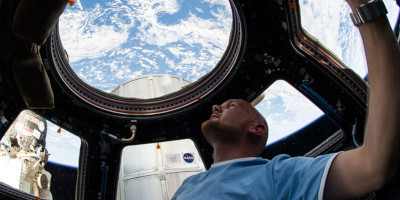
\includegraphics[width=0.3\textwidth]{fb-luftfahrtraumfahrtverkehr}};
    \node [inner sep=0pt] at (0.35\textwidth,-0.2\textwidth) {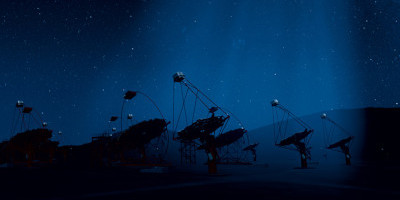
\includegraphics[width=0.3\textwidth]{fb-materie}};
    \node [inner sep=0pt] at (0.7\textwidth,-0.2\textwidth) {
\includegraphics[width=0.3\textwidth]{fb-schluesseltechnologien}};
    \node [fill=desyorange] at (0,0) {\bfseries energy\vphantom{t}};
    \node [fill=desyorange] at (0.35\textwidth,0) {\bfseries earth \& environment};
    \node [fill=desyorange] at (0.7\textwidth,0) {\bfseries health};
    \node [fill=desyorange] at (0,-0.2\textwidth) {\bfseries\parbox{0.16\textwidth}{\centering aeronautics, space \& transport}};
    \node [fill=desyorange] at (0.35\textwidth,-0.2\textwidth) {\bfseries matter};
    \node [fill=desyorange] at (0.7\textwidth,-0.2\textwidth) {\bfseries key technologies};
\end{tikzpicture}
\end{frame}


\begin{frame}
\frametitle{People at DESY}
\vspace*{-2\baselineskip}
\begin{columns}[c]
\column{0.472\textwidth}\begin{itemize}
    \item approximately 2300 employees
    \begin{itemize}
        \item[$\approx\!$] 650 scientists
        \item[$\approx\!$] 700 students, doctoral candidates \& postdocs
        \item[$\approx\!$] 100 young people in commercial and technical training
        \item technical \& administrative staff, \dots
    \end{itemize}
    \item more than 3000 guest scientists from more than 40 countries each year
    \item DESY cooperates closely with many universities and other research centres
    \item DESY operates two student labs to give young people a better understanding of science
\end{itemize}
\column{0.472\textwidth}
    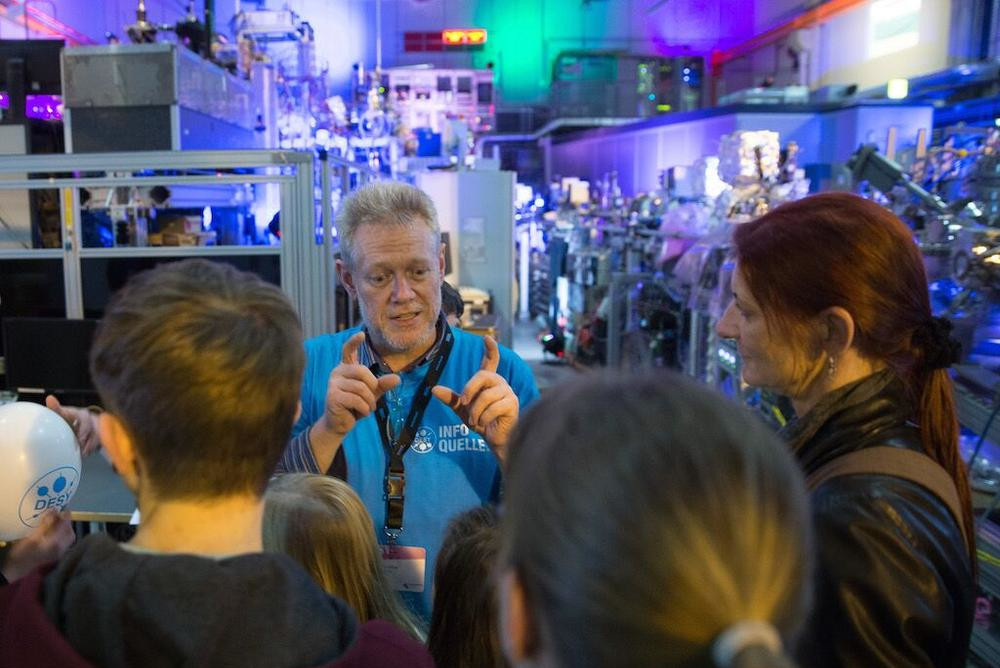
\includegraphics[width=\textwidth]{menschen3} \\[1ex]
    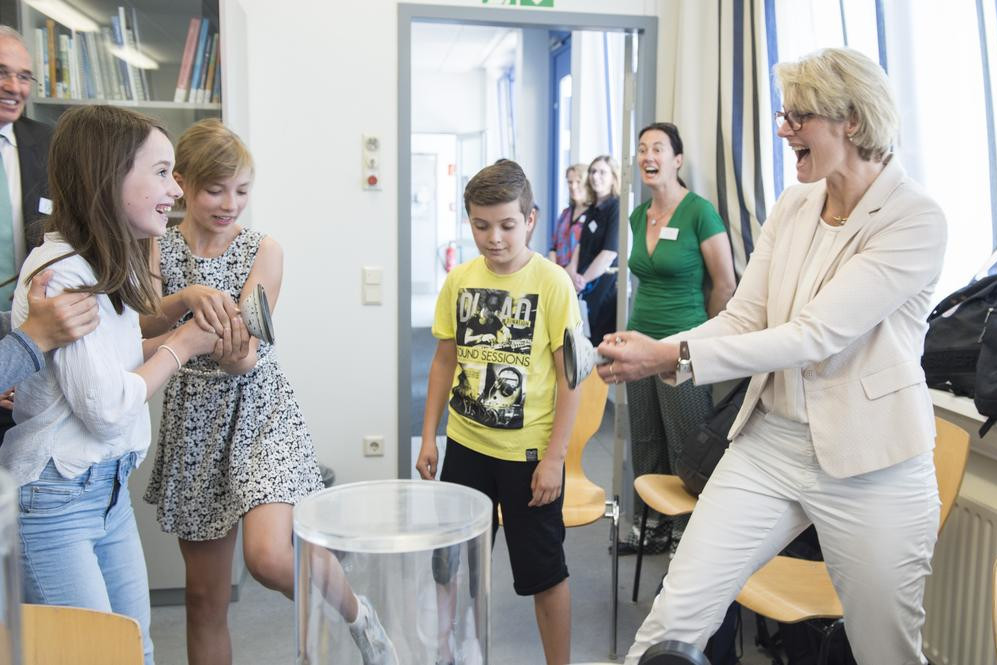
\includegraphics[width=\textwidth]{menschen2} \vspace*{-1cm}
\end{columns}
\end{frame}


\begin{frame}\raggedleft
\frametitle{DESY Campus in Hamburg}
\vspace*{-3.5\baselineskip}
\begin{tikzpicture}
    \node [inner sep=0pt] {\includegraphics[width=0.72\textwidth]{gelaendeplan-hamburg}};
    \node [inner sep=2pt,fill=white] (cfel) at (5.7cm,4cm) {
\includegraphics[width=2cm]{logo-cfel}};
    \node [inner sep=2pt,fill=white,below=0.3cm of cfel] (embl) {
\includegraphics[width=2cm]{logo-embl}};
    \node [inner sep=2pt,fill=white,below=0.3cm of embl] (uhh) {
\includegraphics[width=2cm]{logo-uhh}};
    \node [inner sep=2pt,fill=white,below=0.3cm of uhh] (mpsd) {
\includegraphics[width=2cm]{logo-mpsd}};
    \node [inner sep=2pt,fill=white,below=0.3cm of mpsd] (cssb) {
\includegraphics[width=2cm]{logo-cssb}};
    \node [inner sep=2pt,fill=white,below=0.3cm of cssb] (hzg) {
\includegraphics[width=2cm]{logo-hzg-english}};
    \node [inner sep=2pt,fill=white,below=0.3cm of hzg] (pier) {
\includegraphics[width=2cm]{logo-pier-english}};
    \draw [ultra thick,desyorange,->] (cfel.west) -- (2.6cm,2.3cm);
    \draw [ultra thick,desyorange,->] (embl.west) -- (2.1cm,0.8cm);
    \draw [ultra thick,desyorange,->] (uhh.west) -- (3.5cm,0.5cm);
    \draw [ultra thick,desyorange,->] ($(mpsd.west)!0.2!(mpsd.south west)$) -- (2.8cm,0.2cm);
    \draw [ultra thick,desyorange,->] (cssb.west) -- (1.9cm,0.1cm);
    \draw [ultra thick,desyorange,->] ($(hzg.west)!0.2!(hzg.north west)$) -- (2.6cm,-0.4cm);
    \draw [ultra thick,desyorange,->] ($(pier.west)!0.4!(pier.north west)$) -- (2.2cm,-0.55cm);
    \node [inner sep=0pt] at (-3.5cm,-2.8cm) {\includegraphics[width=0.1\textwidth]{logos/desy}};
\end{tikzpicture}
\vspace*{-13pt}
\end{frame}


\begin{frame}
\frametitle{Research at DESY}
\vspace*{-2\baselineskip}
\begin{tikzpicture}
    \node[inner sep=0pt] at (0,0) {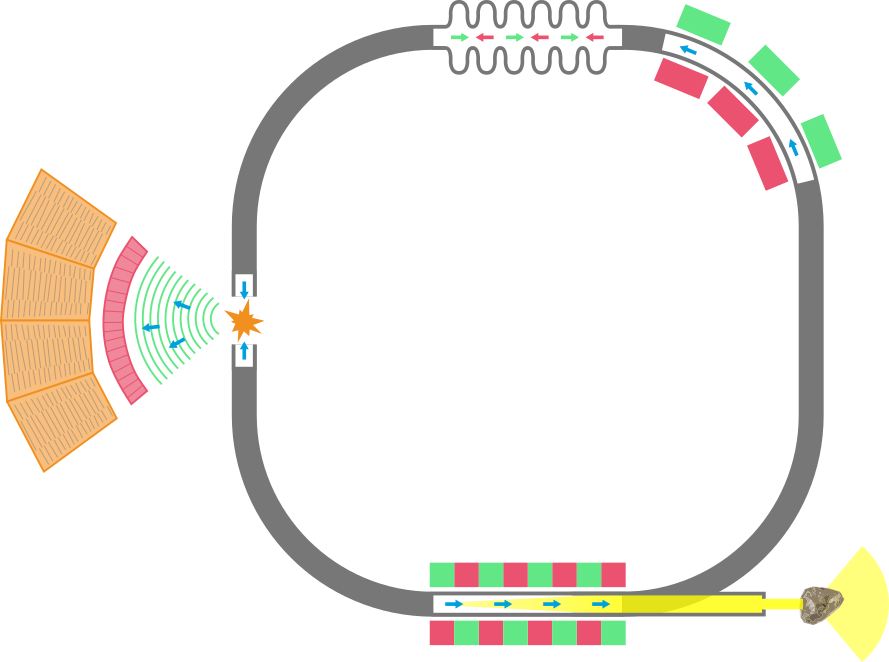
\includegraphics[width=0.9\textwidth]{forschungsgebiete}};
    \node[desyblue] (center) at (1cm,0) {\Large\textbf{Particle Physics}};
    \node[desyblue,above=0.8cm of center] {\Large\textbf{Accelerators}};
    \node[desyblue,below=0.8cm of center] {\Large\textbf{Photon Science}};
\end{tikzpicture}
\vspace*{-11pt}
\end{frame}


\begin{frame}
\frametitle{Accelerators}
\vspace*{-2\baselineskip}
\begin{tikzpicture}
    \node[inner sep=0pt] at (0,0) {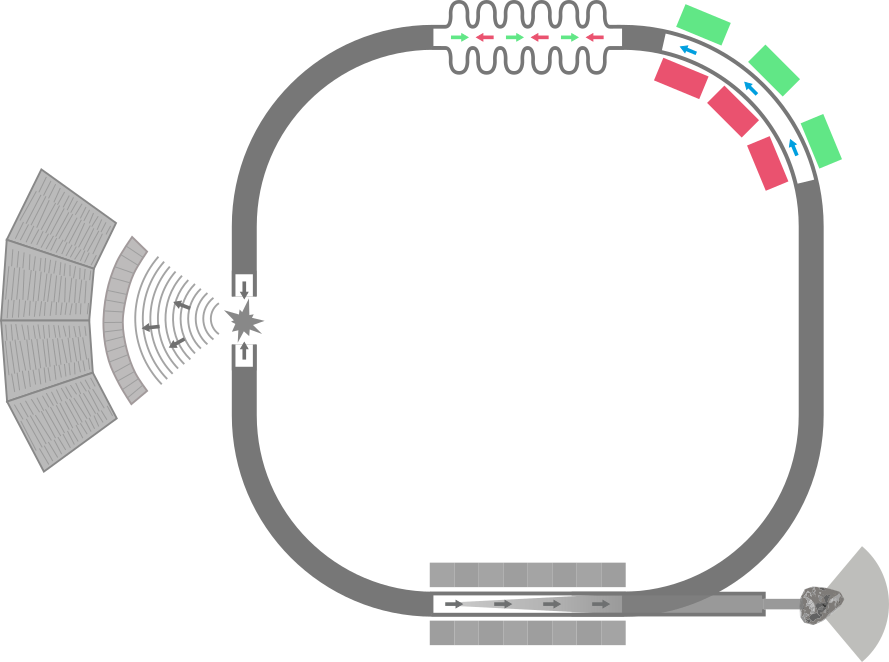
\includegraphics[width=0.9\textwidth]{forschungsgebiete-beschleuniger}};
    \begin{scope}
        \clip [rounded corners=1.5cm] (-1.5cm,-2.4cm) rectangle (3.5cm,2.6cm);
        \node [inner sep=0pt] at (1cm,0.1cm) {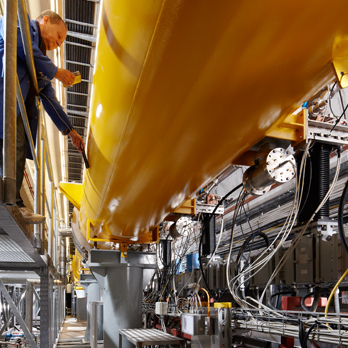
\includegraphics[width=5cm]{gebiet-beschleuniger}};
    \end{scope}
\end{tikzpicture}
\vspace*{-11pt}
\end{frame}


\begin{frame}
\frametitle{Electric and magnetic fields}
\vspace*{-2\baselineskip}
\begin{columns}
\column{0.472\textwidth}\textbf{Electric fields} \\[1em]
\begin{tikzpicture}
    \node [inner sep=0pt] {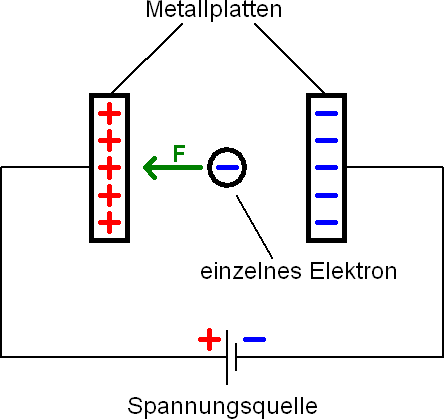
\includegraphics[width=\textwidth]{beschleuniger-efeld}};
    \node [inner sep=2pt,fill=white] at (0cm,2.5cm) {~metal plates~};
    \node [inner sep=2pt,fill=white] at (1cm,-0.8cm) {~~~single electron~~};
    \node [inner sep=2pt,fill=white] at (0cm,-2.5cm) {~~voltage supply~~};
\end{tikzpicture}
\column{0.472\textwidth}\textbf{Magnetic fields} \\[1ex]
    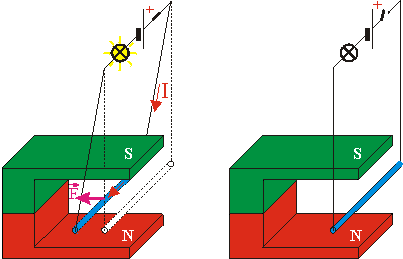
\includegraphics[width=\textwidth]{beschleuniger-lorentzkraft-hufeisen} \\[1em]
    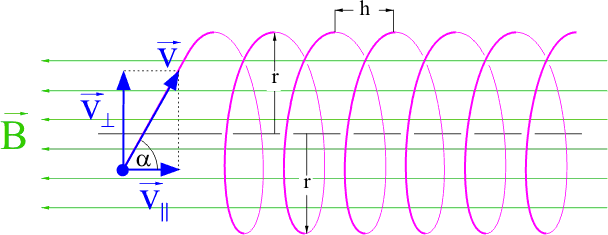
\includegraphics[width=\textwidth]{beschleuniger-lorentzkraft-spirale}
\end{columns}
\vspace*{1em}
\begin{columns}
\column{0.472\textwidth}\centering$\boldsymbol{\Rightarrow}$ \textbf{Acceleration}
\column{0.472\textwidth}\centering$\boldsymbol{\Rightarrow}$ \textbf{Deflection}
\end{columns}
\end{frame}


\begin{frame}
\frametitle{What is a Particle Accelerator?}
\vspace*{-2\baselineskip}
\begin{columns}[c]
\column{0.472\textwidth}\begin{itemize}
    \item goal: particles at high energies
    \begin{itemize}
        \item ``higher energies allow for a study of smaller structures''
        \item mass--energy equivalence: $E=mc^2$ (Einstein, 1905)
    \end{itemize}
    \item accelerate particles with Lorentz force: $\vec{F}=q\Big(\vec{E}+\vec{v}\times\vec{B}\Big)$
    \begin{itemize}
        \item accelerate parallel to electrical field
        \item deviate perpendicular to magnetic field
    \end{itemize}
    \item achieved energies at HERA:
    \begin{itemize}
        \item electrons with 27.5\,GeV $\approx$~99.999\,999\,98\,\% of the speed~of~light
    \end{itemize}
\end{itemize}
\column{0.472\textwidth}\centering
    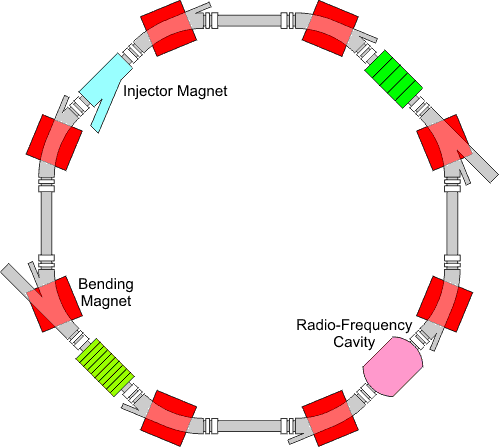
\includegraphics[width=0.8\textwidth]{beschleuniger-schema-en} \\[1em]
    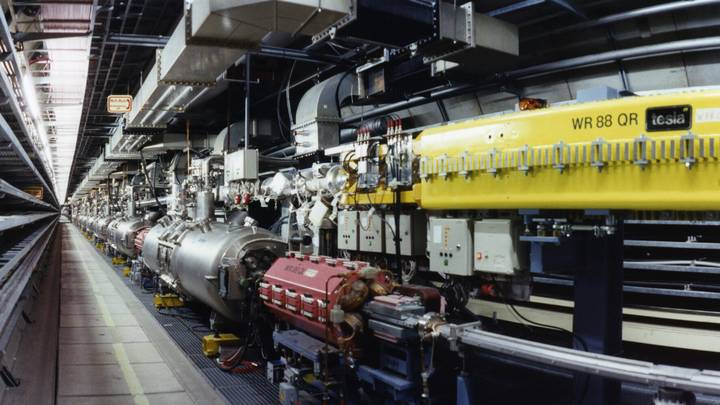
\includegraphics[width=\textwidth,trim={0 0 0 0},clip]{beschleuniger-tunnel}
\end{columns}
\end{frame}


\begin{frame}
\frametitle{Accelerator: \only<1>{DESY}\only<2>{DORIS}\only<3>{PETRA}\only<4>{HERA}\only<5>{FLASH}\only<6>{European XFEL}}
\only<2->{\stepcounter{framenumber}}%
\vspace*{-2\baselineskip}
\begin{tikzpicture}
    \node[inner sep=0pt] at (0,0) {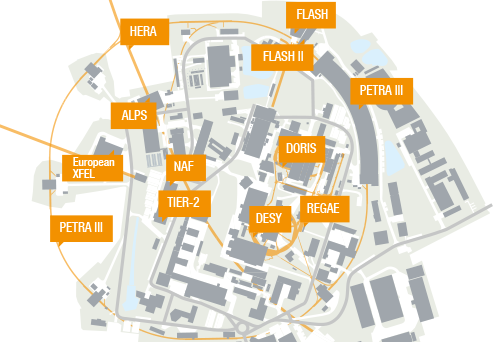
\includegraphics[width=0.9\textwidth]{beschleuniger-desy}};
    \only<1>{\draw [desyblue,line width=3pt] (0.57cm,-1.25cm) circle (0.5cm);}
    \only<2>{\draw [desyblue,line width=3pt,rotate=-15,rounded corners=7pt] (0.45cm,0.35cm) rectangle (1.65cm,0.85cm);}
    \only<3>{\draw [desyblue,line width=3pt] (-0.8cm,-0.2cm) circle (3.5cm);}
    \only<4>{\draw [desyblue,line width=3pt] (-2.9cm,3.6cm) to [bend right=5] (-0.7cm,-1.4cm) to [bend right=13] (1.8cm,-3.6cm);}
    \only<5>{\draw [desyblue,line width=3pt] (0.55cm,1.35cm) -- (1.1cm,3cm) ;}
    \only<6>{\draw [desyblue,line width=3pt] (-2.3cm,-0.15cm) -- (-5.2cm,0.95cm) ;}
    \node [fill=white] at (0.4\textwidth,-1cm) {\parbox{0.28\textwidth}{\raggedright%
        \only<1>{\textbf{D}eutsches \textbf{E}lektronen-\textbf{SY}nchrotron \\[1ex]
        since 1964 \\
        circumference: 317\,m \\
        electrons: 7.4\,GeV}%
        \only<2>{\textbf{DO}ppel-\textbf{R}ing-\textbf{S}peicher \\[1ex]
        from 1974 to 2013 \\
        circumference: 289\,m \\
        electrons: 5\,GeV}%
        \only<3>{\textbf{P}ositron-\textbf{E}lektron-\textbf{T}andem-\textbf{R}ing-\textbf{A}nlage \\[1ex]
        since 1978 \\
        circumference: 2.3\,km \\
        electrons: 6\,GeV (before:~19\,GeV)}%
        \only<4>{\textbf{H}adron-\textbf{E}lektron-\textbf{R}ing-\textbf{A}nlage \\[1ex]
        from 1992 to 2007 \\
        circumference: 6.3\,km \\
        electrons: 27.5\,GeV \\
        protons: 920\,GeV}%
        \only<5>{\textbf{F}reie-Elektronen-\textbf{LAS}er in \textbf{H}amburg \\[1ex]
        since 2005 \\
        length: 315\,m \\
        electrons: 1.2\,GeV}%
        \only<6>{\textbf{X}-Ray \textbf{F}reie-\textbf{E}lektronen-\textbf{L}aser \\[1ex]
        since 2017 \\
        length: 3.4\,km \\
        electrons: 17.5\,GeV}%
    }};
\end{tikzpicture}
\end{frame}


\begin{frame}
\frametitle{Particle Physics}
\vspace*{-2\baselineskip}
\begin{tikzpicture}
    \node[inner sep=0pt] at (0,0) {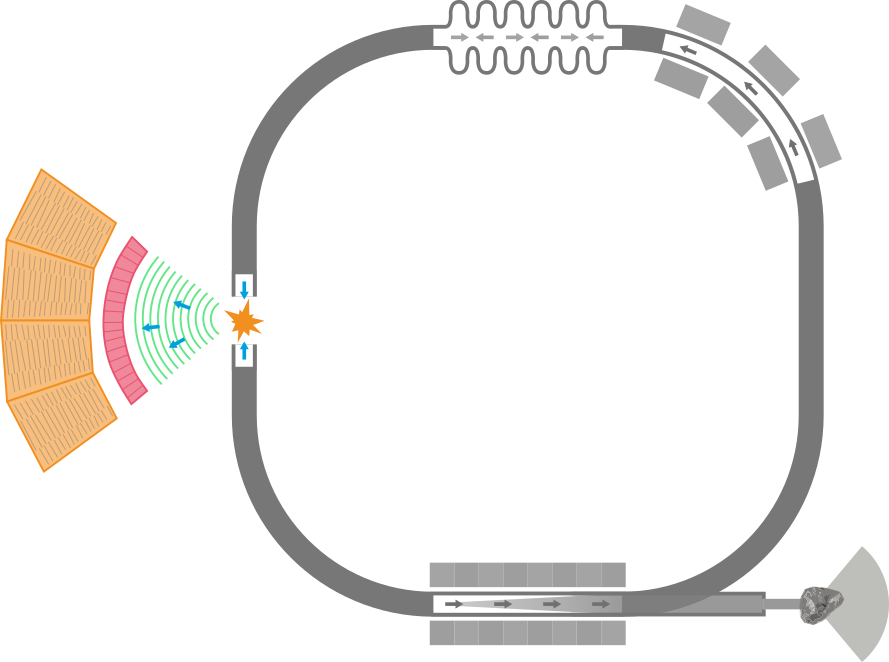
\includegraphics[width=0.9\textwidth]{forschungsgebiete-teilchenphysik}};
    \begin{scope}
        \clip [rounded corners=1.5cm] (-1.5cm,-2.4cm) rectangle (3.5cm,2.6cm);
        \node [inner sep=0pt] at (1cm,0.1cm) {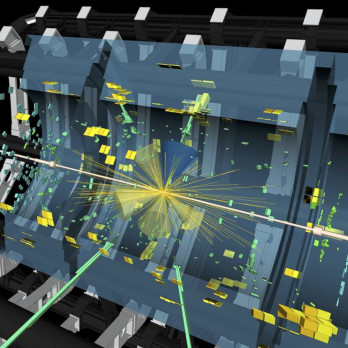
\includegraphics[width=5cm]{gebiet-teilchenphysik}};
    \end{scope}
\end{tikzpicture}
\vspace*{-11pt}
\end{frame}


\begin{frame}
\frametitle{What is Particle Physics?}
\vspace*{-\baselineskip}\normalsize
\begin{tikzpicture}
    \node [inner sep=0pt] {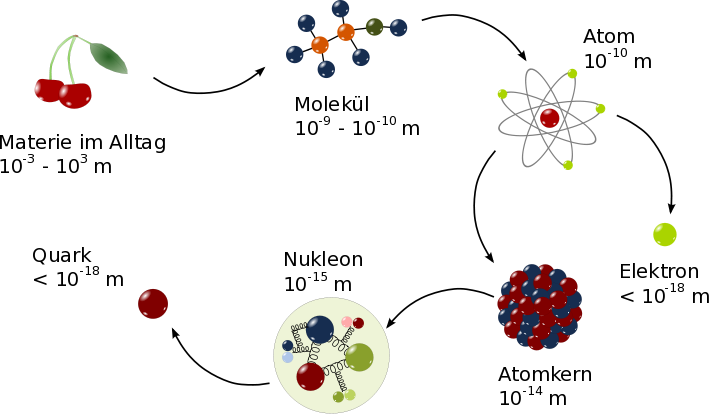
\includegraphics[width=\textwidth]{teilchenphysik-materie}};
    \node [inner sep=2pt,fill=white] (ordinary) at (-4.43cm,1.15cm) {ordinary matter~~~~};
    \fill [white] (ordinary.south east) rectangle (-3.5cm,0.8cm);
    \node [inner sep=2pt,fill=white] at (-0.3cm,1.72cm) {molecule};
    \node [inner sep=2pt,fill=white] at (4.2cm,2.85cm) {atom};
    \node [inner sep=2pt,fill=white] at (5cm,-0.99cm) {electron};
    \node [inner sep=2pt,fill=white] at (3cm,-2.7cm) {atomic nucleus};
    \node [inner sep=2pt,fill=white] at (-0.5cm,-0.86cm) {nucleon};
    \node [inner sep=2pt,fill=white] at (-4.8cm,-0.75cm) {quark};
\end{tikzpicture}
\end{frame}


\begin{frame}\centering
\frametitle{Standard Model of Particle Physics}
\vspace*{-2.5\baselineskip}
\begin{columns}
\column{0.87\textwidth}~\\[-\baselineskip]
    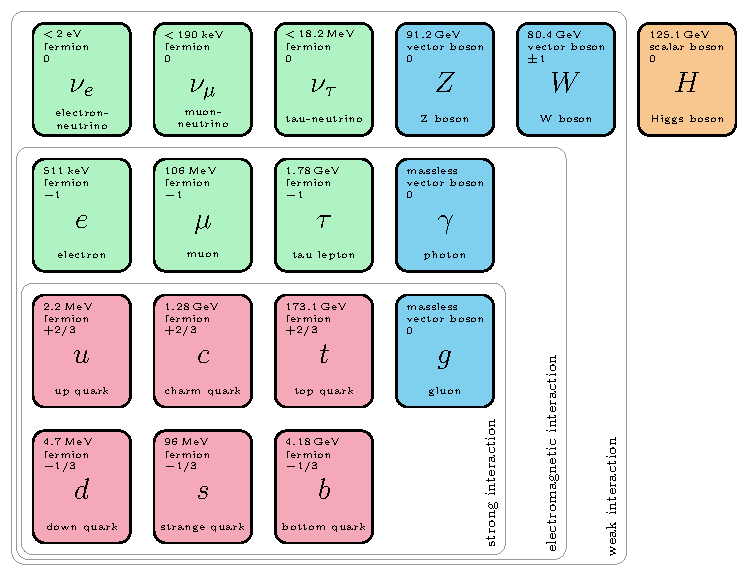
\includegraphics[width=\textwidth]{standardmodell-en}
\column{0.074\textwidth}~\\[4cm]
    \makebox[\textwidth][r]{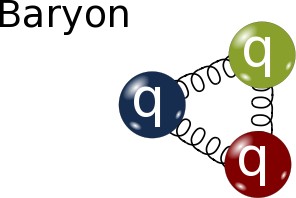
\includegraphics[width=2cm]{teilchenphysik-baryon}} \\[0.5cm]
    \makebox[\textwidth][r]{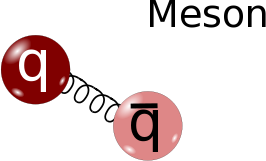
\includegraphics[width=1.8cm]{teilchenphysik-meson}}
\end{columns}

\vspace*{-5pt}
\end{frame}


\begin{frame}
\frametitle{Collider Experiment}
\vspace*{-2\baselineskip}
\begin{columns}
\column{0.151\textwidth}\textbf{Available:}
\column{0.793\textwidth}stable particles \\
    \qquad\textbullet~~ electrons \\
    \qquad\textbullet~~ protons (composed of quarks)
\end{columns}
\vspace*{1ex}
\begin{columns}
\column{0.151\textwidth}\textbf{Interesting:}
\column{0.793\textwidth}rare particles, e.g. Higgs boson, top quark, B meson \\
    \qquad$\Rightarrow$~~ instable, quickly decay to many light particles \\
    \qquad$\Rightarrow$~~ very high mass, i.e. creation requires much energy
\end{columns}
\vspace*{1ex}
\begin{columns}
\column{0.151\textwidth}\textbf{Experiment:}
\column{0.793\textwidth}1. Collide electrons or protons at high energies \\
    \qquad$\Rightarrow$~~ possible to create heavy particles \\[1ex]
    2. Measurement of decay products with large detectors \\
    \qquad$\Rightarrow$~~ reconstruct heavy particles \\
    \qquad$\Rightarrow$~~ perform statistical analysis
\end{columns}
\vspace*{1ex}
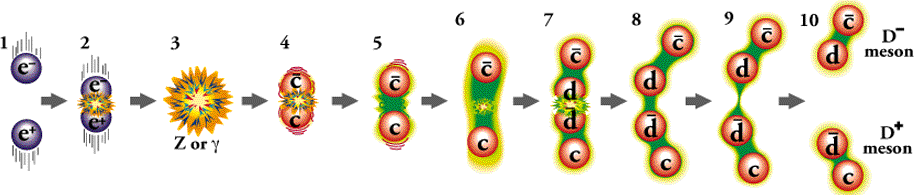
\includegraphics[width=\textwidth]{teilchenphysik-kollision}
\end{frame}


\begin{frame}
\frametitle{Example: CMS Experiment at the LHC}
\vspace*{-2.5\baselineskip}
The \textbf{C}ompact \textbf{M}uon \textbf{S}olenoid experiment is one of the four experiments at the \textbf{L}arge \textbf{H}adron \textbf{C}ollider, the world's largest accelerator, at CERN. \\[\baselineskip]
\makebox[\textwidth]{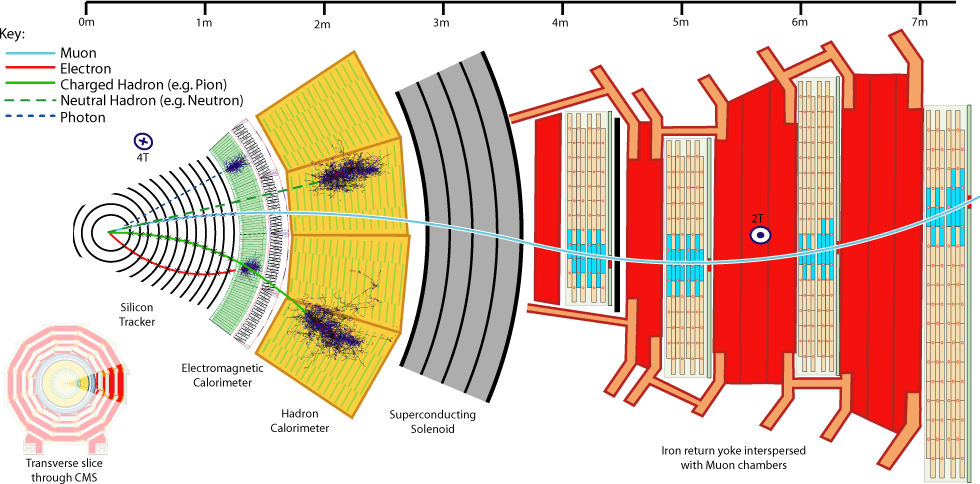
\includegraphics[width=0.99\paperwidth]{teilchenphysik-detektor}}
\vspace*{-18pt}
\end{frame}


\begin{frame}
\frametitle{Gluon Discovery at PETRA}
\vspace*{-2.6\baselineskip}
\alert{\bfseries\footnotesize R. Brandelik et al. (TASSO Collaboration), Evidence for planar events in e\textsuperscript{+}e\textsuperscript{--} annihilation at high energies, Physics Letters 86B, 243--249 (1979)}
\vspace*{\baselineskip}
\begin{columns}
\column{0.2\textwidth}
    \textbf{only quarks} \\
    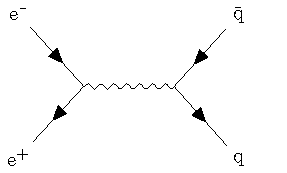
\includegraphics[width=\textwidth,page=1]{gluon-feynman} \\[1ex]
    \textbf{with gluons} \\
    \includegraphics[width=\textwidth,page=2]{gluon-feynman} \\
    \includegraphics[width=\textwidth,page=3]{gluon-feynman} \\
    \includegraphics[width=\textwidth,page=4]{gluon-feynman}
\column{0.744\textwidth}PETRA experiments observed events with three jets, which could not be explained with a quark-only theory $\Rightarrow$ the gluon was discovered \\[1ex]
    \centering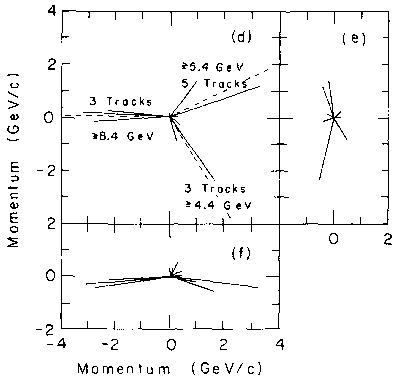
\includegraphics[width=0.7\textwidth]{gluon-threejets}
\end{columns}
\vspace*{-18pt}
\end{frame}


\begin{frame}
\frametitle{Proton Structure at HERA}
\vspace*{-2.6\baselineskip}
\alert{\bfseries\footnotesize H. Abramowicz et al. (H1 and ZEUS Collaborations), Combination of measurements of inclusive deep inelastic e\textsuperscript{$\pm$}p scattering cross sections and QCD analysis of HERA data, European Physical Journal C75 (2015) 12, 580}
\vspace*{\baselineskip}
\begin{columns}
\column{0.472\textwidth}~\\[-\baselineskip]
\begin{minipage}[c]{0.3\textwidth}
    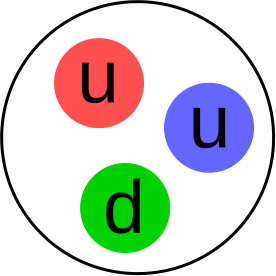
\includegraphics[width=\textwidth]{hera-proton1}
\end{minipage}
\hfill
\begin{minipage}[c]{0.65\textwidth}\raggedright
    The proton consists of three ``valence'' quarks: two up quarks and one down quark.
\end{minipage}\vspace*{1ex}

However, the quarks interact via the strong interaction constantly, such that gluons as well as other quarks and anti-quarks can be found inside the proton.

\begin{minipage}[c]{0.35\textwidth}
    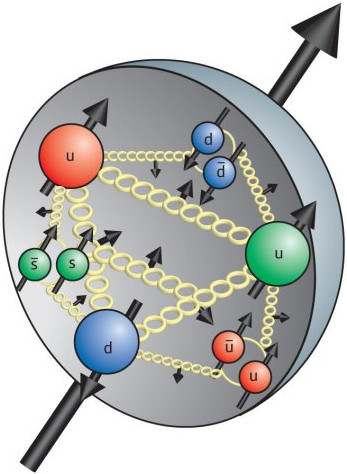
\includegraphics[width=\textwidth]{hera-proton2}
\end{minipage}
\hfill
\begin{minipage}[c]{0.6\textwidth}\raggedright
    At HERA, the composition of the proton was measured with such a high precision, that the results will be the best available for a long time.
\end{minipage}
\column{0.472\textwidth}~\\[-\baselineskip]
    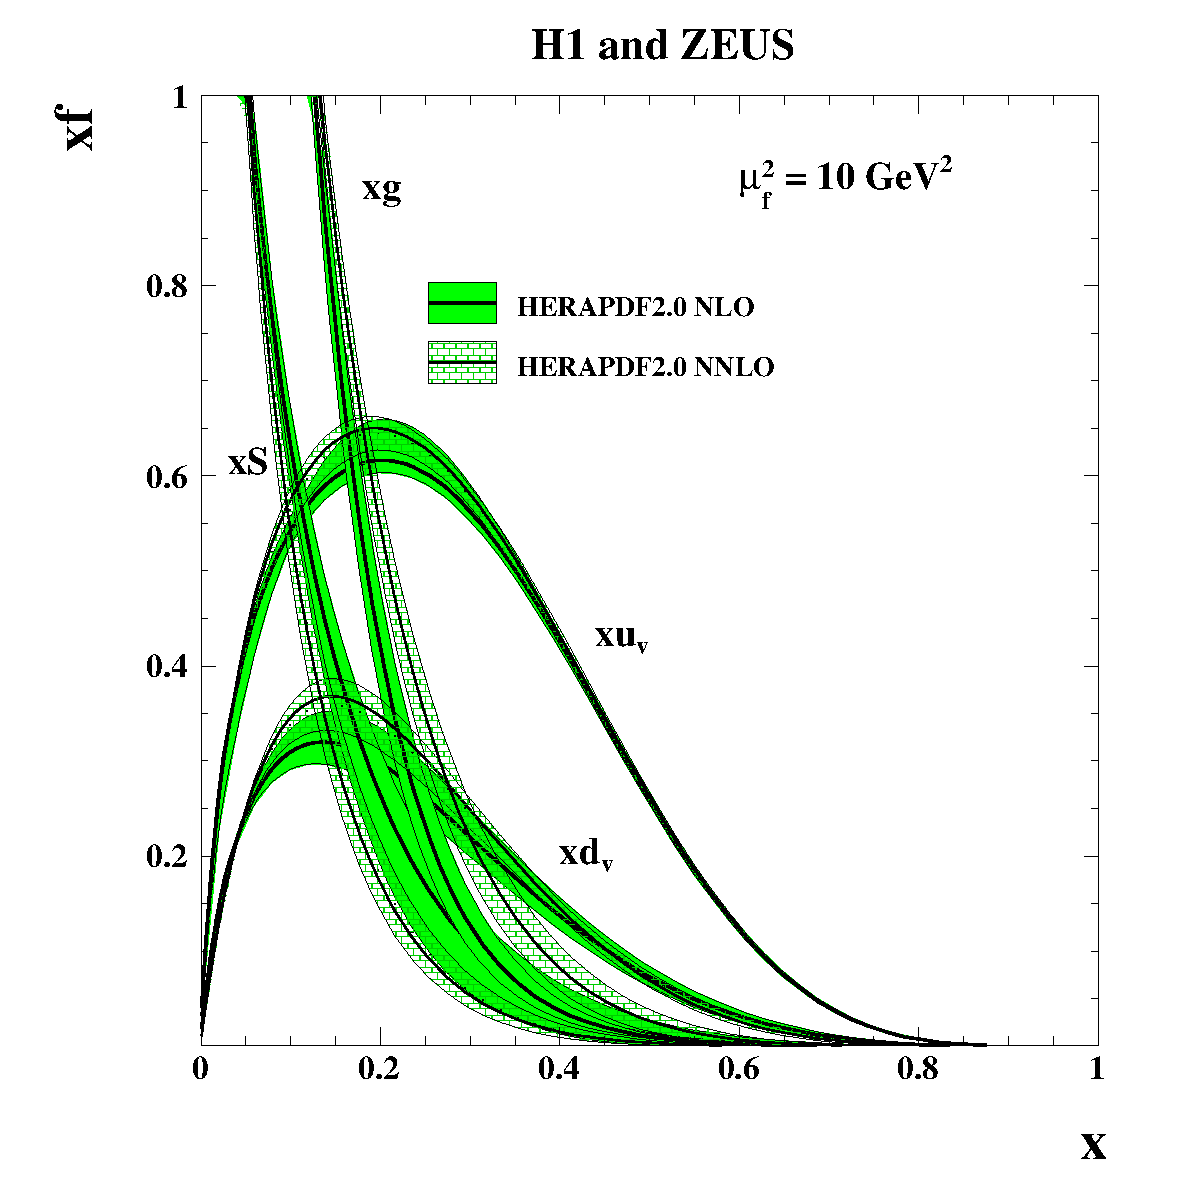
\includegraphics[width=\textwidth,trim={2.4cm 1.7cm 1.1cm 0.4cm},clip]{hera-pdf}
\end{columns}
\vspace*{-7pt}
\end{frame}


\begin{frame}
\frametitle{Observation of $\boldsymbol{H\rightarrow b\bar{b}}$ at the LHC}
\vspace*{-2.6\baselineskip}
\alert{\bfseries\footnotesize M. Aaboud et al. (ATLAS Collaboration), Observation of $\boldsymbol{H\rightarrow b\bar{b}}$ decays and $\boldsymbol{VH}$ production with the ATLAS detector, Physics Letters B786 (2018) 59--86}
\vspace*{\baselineskip}
\begin{columns}
\column{0.472\textwidth}\centering~\\[-\baselineskip]
    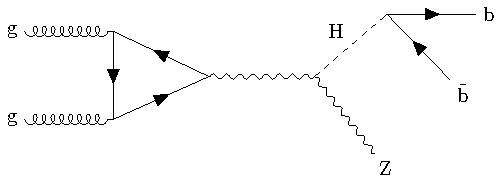
\includegraphics[width=\textwidth]{vhbb-feynman} \\[1ex]
    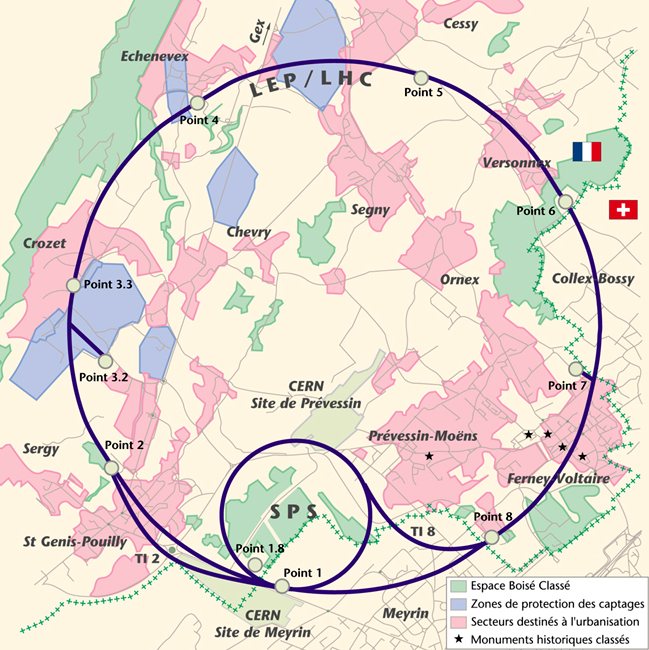
\includegraphics[width=0.8\textwidth]{vhbb-lhc}%
    \Put(-15,53){\includegraphics[width=0.6cm]{logos/cms}}%
    \Put(-23,15){\setlength\fboxsep{0pt}\fbox{
\includegraphics[height=0.5cm]{vhbb-atlas}}}
\column{0.472\textwidth}~\\[-\baselineskip]
    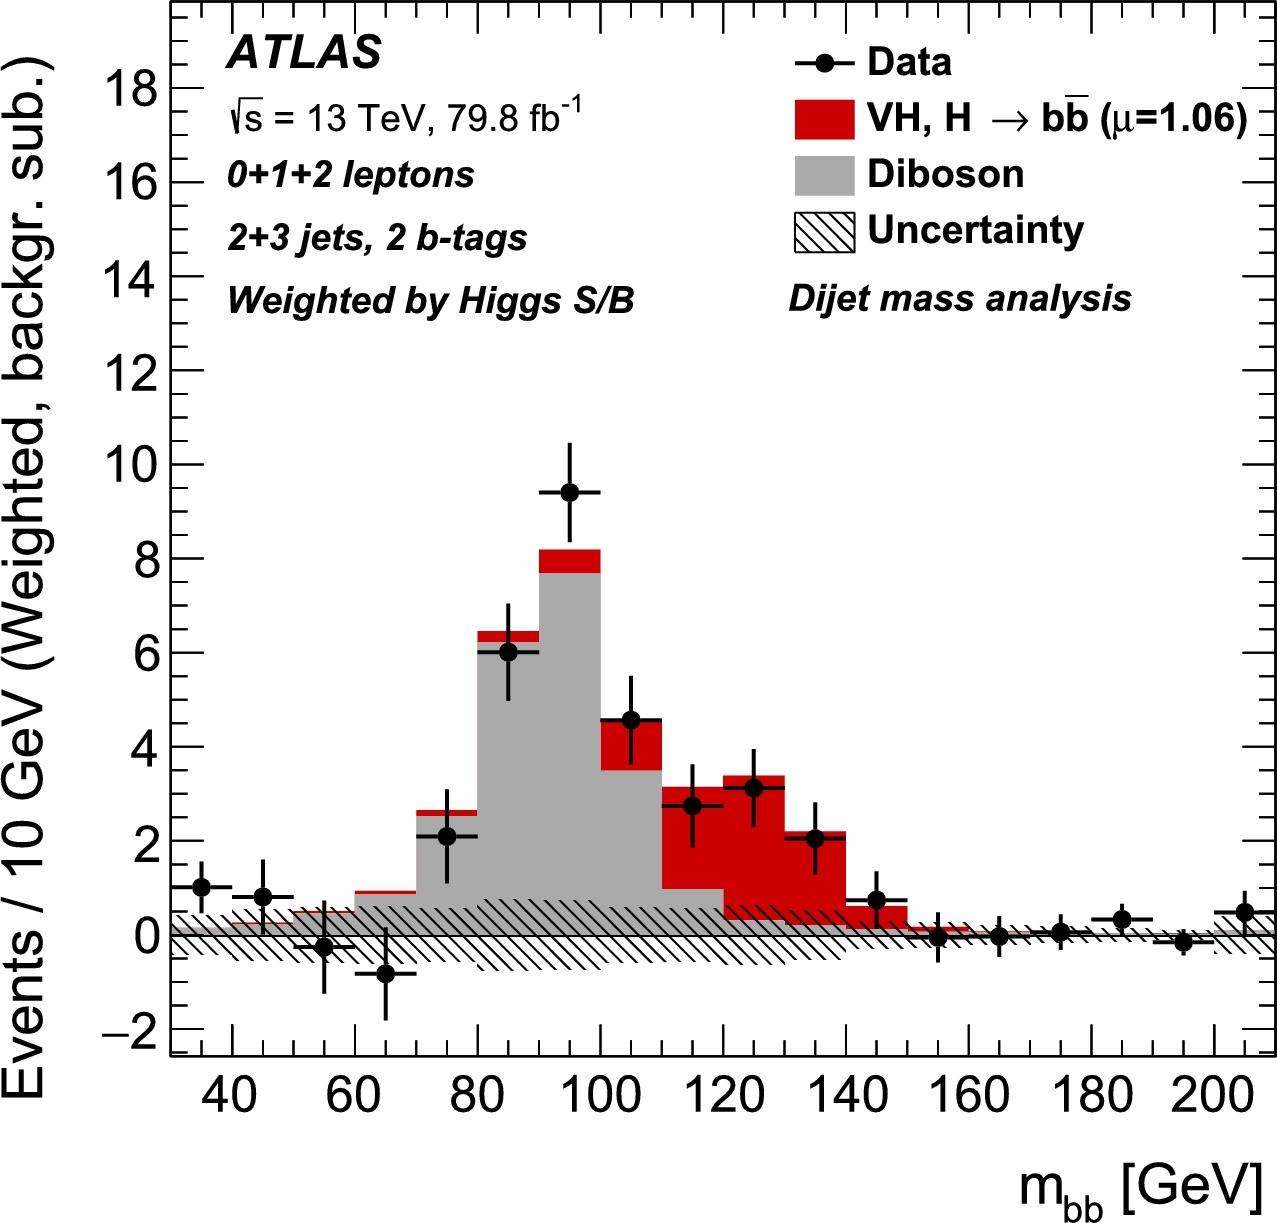
\includegraphics[width=\textwidth]{vhbb-result} \\[1ex]
    $H\rightarrow b\bar{b}$ can only be distinguished from $Z\rightarrow b\bar{b}$ by a statistical analysis.
\end{columns}
\vspace*{-3pt}
\end{frame}


\begin{frame}
\frametitle{High-Energetic Neutrinos with IceCube}
\vspace*{-2.6\baselineskip}
\alert{\bfseries\footnotesize M. Aartsen et al. (IceCube Collaboration), Neutrino emission from the direction of the blazar TXS 0506+056 prior to the IceCube-170922A alert, Science 361 (2018) 6398}
\vspace*{\baselineskip}
\begin{columns}
\column{0.472\textwidth}\textbf{Experiment} \\[1ex]
    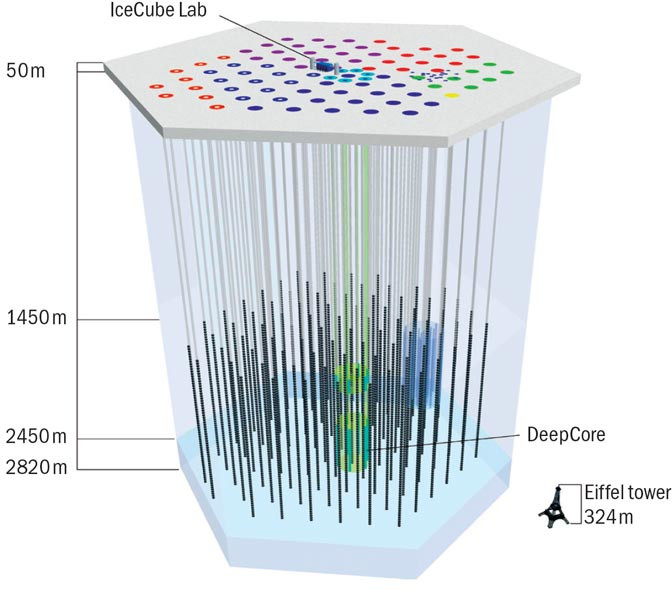
\includegraphics[width=\textwidth]{icecube-experiment} \\
    Neutrino observatory with 5160 sensors built into one cubic kilometer of ice at the south pole
\column{0.472\textwidth}\textbf{Measurement} \\[1ex]
    \includegraphics[width=\textwidth]{icecube-ergebnis} \\
    first detection of neutrino with energy of 300\,TeV from blazar about 4 billion light years away from earth $\Rightarrow$ confirmed by other astrophysical observations
\end{columns}
\vspace*{-8pt}
\end{frame}


\begin{frame}
\frametitle{Photon Science}
\vspace*{-2\baselineskip}
\begin{tikzpicture}
    \node[inner sep=0pt] at (0,0) {\includegraphics[width=0.9\textwidth]{forschungsgebiete-forschungmitphotonen}};
    \begin{scope}
        \clip [rounded corners=1.5cm] (-1.5cm,-2.4cm) rectangle (3.5cm,2.6cm);
        \node [inner sep=0pt] at (1cm,0.1cm) {\includegraphics[width=5cm]{gebiet-forschungmitphotonen}};
    \end{scope}
\end{tikzpicture}
\vspace*{-11pt}
\end{frame}


\begin{frame}
\frametitle{Accelerators as Light Sources}
\vspace*{-2.2\baselineskip}
\begin{columns}
\column{0.562\textwidth}~\\[-\baselineskip]
\makebox[\textwidth][l]{\begin{tikzpicture}
    \node [inner sep=0pt] at (0,0) {\includegraphics[width=1.4\textwidth]{photonen-erzeugung}};
    \node [inner sep=1pt,fill=white] at (-3.3cm,1.88cm) {\footnotesize bending magnet};
    \node [inner sep=1pt,fill=white] at (-3.5cm,-0.2cm) {\footnotesize wiggler};
    \node [inner sep=1pt,fill=white] at (-3.4cm,-2.2cm) {\footnotesize undulator};
    \node [inner sep=1pt,fill=white] at (-2.75cm,-3.7cm) {\footnotesize free-electron laser~~~};
\end{tikzpicture}}
\column{0.382\textwidth}~\\ charged particles bent on a circular track emit light
\begin{itemize}
    \item ``synchrotron radiation''
    \item very intensive and highly focussed light
\end{itemize}
\end{columns}
\vspace*{-7pt}
\end{frame}


\begin{frame}
\frametitle{Experiments with Light}
\vspace*{-1.5\baselineskip}
\begin{tikzpicture}
    \node [inner sep=0pt] {\includegraphics[width=\textwidth]{photonen-experiment}};
    \node [shape=circle,draw,fill=white,inner sep=2pt] at (-4cm,2.5cm) {1};
    \node [shape=circle,draw,fill=white,inner sep=2pt] at (-2.17cm,2.5cm) {2};
    \node [shape=circle,draw,fill=white,inner sep=2pt] at (0.8cm,2.5cm) {3};
    \node [shape=circle,draw,fill=white,inner sep=2pt] at (4.7cm,-1.7cm) {4};
    \node [inner sep=0pt] at (-3cm,-2.5cm) {\parbox{5.5cm}{\raggedright\begin{enumerate}
        \item The electron beam emits light in magnetic structures.
        \item The object is irradiated.
        \item Scattered/emitted/non-absorbed light is measured.
        \item The object's structure is \makebox[0pt][l]{reconstructed}\\ from the measured data.
    \end{enumerate}}};
    \node [inner sep=0pt] at (3.8cm,1.2cm) {\parbox{4cm}{\raggedright%
        \textbf{Spectroscopy} measures chemical processes from emission and absorption spectra. \\[1ex]
        \textbf{Diffraction} measures atomic structures from light bending at crystalls. \\[1ex]
        \textbf{Imaging} recreates structures as in an ordinary microscope.
    }};
\end{tikzpicture}
\vspace*{-22pt}
\end{frame}


\begin{frame}
\frametitle{PETRA III \color{desyorange}\large -- most brilliant light source of its kind}
\vspace*{-2\baselineskip}
\begin{tikzpicture}
    \node [inner sep=0pt] {\includegraphics[width=0.78\textwidth]{photonen-petra3}};
    \node [inner sep=3pt,fill=white] at (3cm,-3cm) {\parbox{7.6cm}{\raggedright\small%
        electron energy: 6\,GeV \\
        photon energy: 150\,eV\,--\,200\,keV \\
        photon wavelength: 8\,nm\,--\,0.006\,nm \\
        peak brilliance: 10\textsuperscript{21}\,ph\,/\,(s\,mm\textsuperscript{2}\,mrad\textsuperscript{2}\,0.1\,\%\,BW)
    }};
\end{tikzpicture}
\vspace*{-4pt}
\end{frame}


\begin{frame}
\frametitle{FLASH \color{desyorange}\large -- world's first soft X-ray free-electron laser}
\vspace*{-2\baselineskip}
\begin{tikzpicture}
    \node [inner sep=0pt] {\includegraphics[width=0.75\textwidth]{photonen-flash}};
    \node [inner sep=3pt,fill=white] at (3.5cm,-3.7cm) {\parbox{7.3cm}{\raggedright\small%
        electron energy: 0.35\,GeV\,--\,1.25\,GeV \\
        photon energy: 14\,eV\,--\,310\,eV \\
        photon wavelength: 90\,nm\,--\,4\,nm \\
        pulse duration: 30\,fs\,--\,200\,fs \\
        peak brilliance: 10\textsuperscript{31}\,ph\,/\,(s\,mm\textsuperscript{2}\,mrad\textsuperscript{2}\,0.1\,\%\,BW)
    }};
\end{tikzpicture}
\vspace*{-22pt}
\end{frame}


\begin{frame}
\frametitle{European XFEL \color{desyorange}\large -- largest X-ray laser in the world}
\vspace*{-2\baselineskip}
\includegraphics[width=\textwidth]{photonen-xfel}%
\Put(-10,10){\includegraphics[width=0.07\textwidth]{logos/desy}}%
\Put(-85,10){\includegraphics[width=0.07\textwidth]{logo-xfel}}
\vspace*{1ex}\small

electron energy: up to 17.5\,GeV \\
photon energy: from 0.2\,keV to at least 25\,keV  \\
photon wave length: from 4.7\,nm to at least 0.05\,nm \\
pulse duration: less than 100\,fs \\
peak brilliance: 5\,$\times$\,10\textsuperscript{33}\,ph\,/\,(s\,mm\textsuperscript{2}\,mrad\textsuperscript{2}\,0.1\,\%\,BW)
\end{frame}


\begin{frame}
\frametitle{``FLASH, what a picture!''}
\vspace*{-2.6\baselineskip}
\alert{\bfseries\footnotesize H. Chapman et al., Femtosecond diffractive imaging with a soft-X-ray free-electron laser, Nature Physics 2, 839--843 (2006)}
\vspace*{\baselineskip}
\begin{columns}[c]
\column{0.472\textwidth}\includegraphics[width=\textwidth]{flash-aufbau}
\column{0.472\textwidth}\begin{itemize}
    \item sample with \textmu m structure illuminated with single X-ray laser pulse
    \item diffraction pattern recorded with CCD sensor (at different angles by use of multilayer mirror)
\end{itemize}
\end{columns}
\vspace*{1ex}
\begin{columns}[c]
\column{0.25\textwidth}\includegraphics[width=\textwidth]{flash-beugungsbild}
\column{0.3\textwidth}\begin{itemize}
    \item left: recorded diffraction pattern
    \item right: reconstructed X-ray image
    \item first demonstration of high-resolution imaging with FLASH
\end{itemize}
\column{0.35\textwidth}\includegraphics[width=\textwidth]{flash-rekonstruiert}
\end{columns}
\vspace*{-3pt}
\end{frame}


\begin{frame}
\frametitle{Biochemistry: Ribosome Structure}
\vspace*{-2.6\baselineskip}
\alert{\bfseries\footnotesize A. Tocilj et al., The small ribosomal subunit from \textit{Thermus thermophilus} at 4.5\,\AA{} resolution: Pattern fittings and the identification of a functional site, Proc. Natl. Acad. Sci. USA 95 (1999) 25, 14252--14257}
\vspace*{\baselineskip}
\begin{columns}
\column{0.492\textwidth}~\\[-\baselineskip]
    \includegraphics[width=\textwidth]{ribosom-struktur}
    \vspace*{-1ex}

    \begin{minipage}[c]{0.2\textwidth}
        \includegraphics[width=\textwidth]{nobelpreis}
    \end{minipage}
    \hfill
    \begin{minipage}[c]{0.75\textwidth}\raggedright\footnotesize
        Nobel prize in chemistry 2009 to Ada Yonath ``for studies of the structure and function of the ribosome''
    \end{minipage}
\column{0.452\textwidth}~\\[-\baselineskip]
    \includegraphics[width=\textwidth]{ribosomen-messung}
\end{columns}
\vspace*{-7pt}
\end{frame}


\begin{frame}
\frametitle{Nanoparticles: Catalyst Studies}
\vspace*{-2.6\baselineskip}
\alert{\bfseries\footnotesize U. Hejral et al., Identification of a catalytically highly active surface phase for CO oxidation over PtRh nanoparticles under operando reaction conditions, Physical Review Letters 120, 126101 (2018)}
\vspace*{\baselineskip}
\begin{columns}
\column{0.532\textwidth}~\\[-\baselineskip]
    \includegraphics[width=\textwidth]{nano-methode}
\column{0.412\textwidth}study of reactivity of CO\,$\rightarrow$\,CO\textsubscript{2} oxidation in presence of Pt--Rh alloy nanoparticle catalyst
    \vspace*{1ex}
    
    result: the more edges, the higher the reactivity
    \vspace*{1ex}

    \includegraphics[width=\textwidth]{nano-3d}
\end{columns}
\end{frame}


\begin{frame}
\frametitle{Art: Hidden Paintings}
\vspace*{-2.6\baselineskip}
\alert{\bfseries\footnotesize J. Dik et al., Visualization of a lost painting by Vincent van Gogh using synchrotron radiation based X-ray fluorescence elemental mapping, Anal. Chem. 80 (2008) 16}
\vspace*{0.5\baselineskip}
\begin{columns}
\column{0.472\textwidth}\textbf{Original: \glqq Patch of Grass\grqq\\(Vincent van Gogh)} \\[1ex]
    \includegraphics[width=\textwidth]{vangogh-original}
\column{0.472\textwidth}\textbf{Reconstruction of hidden picture from fluorescence measurements} \\[1ex]
    \includegraphics[width=\textwidth]{vangogh-rekonstruktion}
\end{columns}
\vspace*{-8pt}
\end{frame}


\usebackgroundtemplate{\includegraphics[width=\paperwidth]{desygelaende}}
\begin{frame}[plain]
\vspace*{0.72\paperheight}
\setlength\fboxsep{0.044\paperwidth}
\makebox[\dimexpr3.5cm+\fboxsep][r]{\colorbox{white}{\parbox{\dimexpr3.5cm}{%
    \emph{\bfseries Have fun at the tour!} \\[1ex]
    \textbullet~~ Take fotos! \\
    \textbullet~~ Ask questions!
}}}%
\Put(-34,60){\includegraphics[width=1.5cm]{logo-herab}}%
\Put(38,100){\setlength\fboxsep{0pt}\fbox{\includegraphics[width=3cm]{logo-petra3}}}%
%\Put(8,38){\includegraphics[width=0.5cm]{locator}}% SR 3,4,5
%\Put(-1,25){\includegraphics[width=0.5cm]{locator}}% SR 1,1b
%\Put(22,14){\includegraphics[width=0.5cm]{locator}}% Hörsaal, Geb. 5
%\Put(58,30){\includegraphics[height=0.5cm]{locator2}}% 3/BAH1
\end{frame}



\end{document}